\chapter{Sensor Inertial Mesure Unit}

Inertial Measurement Units (IMU) are an essential component of many navigation and control systems. These devices integrate several sensors, including accelerometers and gyroscopes, to measure and track an object's movements in three-dimensional space. IMUs are widely used in a variety of applications, such as autonomous vehicle navigation, virtual reality, image stabilization, and even in wearable devices for tracking physical activity. Their ability to provide precise data on linear and angular acceleration makes them indispensable tools for systems requiring precise control and orientation, and ongoing technological advances have reduced their size, power consumption and cost, widening their scope of application in many fields. 
\cite{st_lsm9ds1:2025} \cite{analogdevices:2024} 


\section{General Description }

The Inertial Measurement Unit is used to mesured acceleration or rotation, this is an electronic device which used three types of sensor magnetometer, accelerometer and gyroscope. These three sensors is used in LSM9DS1 and they give velocity, orientation and gravital force. 

The magnetometer measures the strength of magnetic fields, providing various types of information. For instance, when you pass a current through an electromagnet or generate a magnetic field in another way, the magnetometer can detect and quantify the strength of that field. \cite{st_microelectronics:2024}
\cite{STMicroelectronics_LSM9DS1:2024}

\subsection{Always On Mode}

This feature implies that the LSM9DS1 can remain operational continuously, even when a device is in sleep mode, without excessively draining power. Such functionality proves invaluable for applications that require uninterrupted motion tracking, like fitness monitoring or navigation systems. \cite{st_microelectronics:2024}

\bigskip

The power consumption is an important factor when we have battery-powered device like smartphone. These devices need to be lightweight and portable, which requires minimizing battery weight and maximizing battery life.

\bigskip

The LSM9DS1 consumes only 0.55 mA when operating in combo high-performance mode. This low power consumption allows the sensor to deliver exceptional data quality while efficiently using battery power. In this mode, the sensor can simultaneously measure acceleration and angular rate, providing precise and reliable data even at high sampling rates.


\subsection{Tilt detection}

These features imply that tilt detection relies on the accelerometer to detect movement. When movement occurs, the tilt detection feature identifies it. Additionally, the tilt function operates with ultra-low power consumption. \cite{st_microelectronics:2024}

For example, if you have your smartphone in your front pant pocket, the tilt detection feature can determine whether you are moving from a standing to a sitting position or from sitting to standing.

\subsection{Significant Motion Detection}

This feature indicates that the Significant Motion Detection in the LSM9DS1 uses only the accelerometer to detect large movements.\cite{st_microelectronics:2024}

\section{Specific Sensor }
\subsection{LSM9DS1}

The LSM9DS1 sensor, engineered by STMicroelectronics, is a highly advanced 3-axis Inertial Measurement Unit (IMU) that incorporates a high-performance 3-axis digital accelerometer and 3-axis digital gyroscope. This meticulously crafted device is designed for precise motion tracking and finds extensive use in wearable devices and smartphones. With its capability to concurrently measure both linear and rotational motion, it stands as a benchmark in motion-sensing technology. \cite{STMicroelectronics_LSM9DS1:2024}

Developed to detect various types of motion, the LSM9DS1 sensor offers features such as stationary/motion detection, tilt sensing, pedometer functions, and timestamping. Additionally, it supports the integration of an external magnetometer, expanding its functionality further. The sensor provides hardware flexibility, allowing for different pin connections to external sensors. This flexibility enables the expansion of functionalities, such as adding a sensor hub or auxiliary SPI connections, to meet diverse application requirements.

\bigskip

\subsection{Accelerometer}

The STMicroelectronics LSM9DS1 accelerometer is an advanced sensor crafted to measure linear acceleration along the x, y, and z axes. Its wide measurement range, spanning from ±2g to ±16g, ensures versatility across various applications. Boasting exceptional precision and reliability, it stands as a go-to choice for engineers and designers seeking accurate motion tracking solutions. \cite{STMicroelectronics_LSM9DS1:2024}
\bigskip 

Moreover, its low power consumption, typically ranging from 0.55 mA to 1.25 mA, makes it ideal for battery-powered devices. This feature ensures prolonged operation without draining excessive power, enhancing the efficiency and longevity of battery-powered systems.

\bigskip 

With an operating voltage range of 1.71 V to 3.6 V, the LSM9DS1 accelerometer easily adapts to different system configurations, offering flexibility in integration. Whether employed in wearable devices for motion tracking, drones for stabilization, or structural monitoring for vibration analysis, the LSM9DS1 accelerometer consistently delivers outstanding performance.

\bigskip 

Compact yet robust, the LSM9DS1 accelerometer is engineered to withstand demanding environments while providing precise and reliable measurements. Its reputation as a preferred choice among engineers and designers underscores its ability to meet the stringent requirements of diverse projects.

\bigskip 

\begin{center}
	
	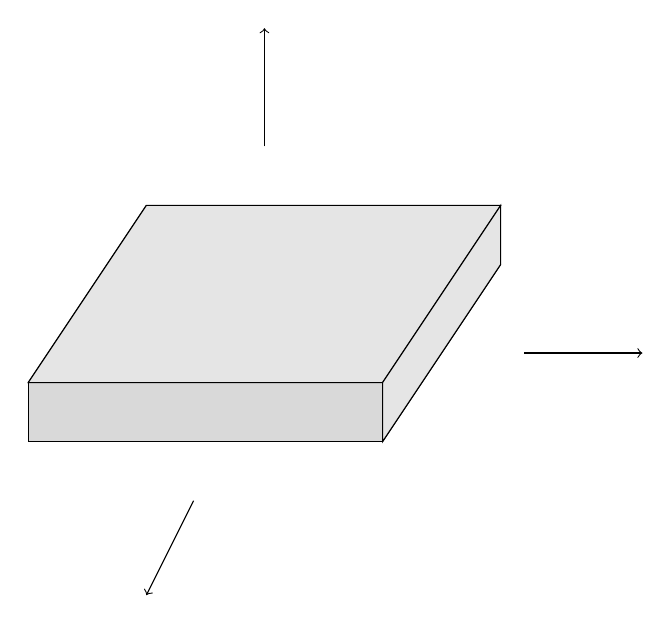
\begin{tikzpicture}[scale=1.5]
		% Face avant
		\draw[fill=gray!30] (0,0) rectangle (3,0.5);
		
		\draw (0,0.5) -- (1,2);
		\draw (3, 0.5) -- (4,2);
		\draw (3,0) -- (4,1.5);
		\draw (4,1.5) -- (4,2);
		\draw (1,2) -- (4,2);
		\draw[fill=gray!20] (0,0.5) -- (3,0.5) -- (4,2) -- (1,2) -- cycle;
		\draw[->] (2, 2.5) -- (2, 3.5);
		\draw[->] (4.2, 0.75) -- (5.2, 0.75);
		\draw[->] (1.4,- 0.5) -- (1,-1.3);
		\draw[fill=gray!20] (3,0) -- (3,0.5) -- (4,2) -- (4,1.5) -- cycle;			
	\end{tikzpicture}
	
	\begin{figure}[H]
		\caption{LSM9DS1 axis  on this card}
	\end{figure}
	
\end{center}

\subsection{Gyroscope}

The STMicroelectronics LSM9DS1 gyroscope is a sophisticated measuring instrument designed to assess rotation rates around the x, y, and z axes. With a typical measurement range of ±245/500/2000 dps, it offers great flexibility to adapt to the specific needs of various applications. \cite{STMicroelectronics_LSM9DS1:2024}

\bigskip 

Operating within a voltage range of 1.71 V to 3.6 V, this gyroscope can seamlessly integrate into different system configurations. Furthermore, its typical operating current ranges from 1 mA to 2 mA, ensuring optimal energy efficiency for battery-powered devices.

\bigskip 

Whether it's for inertial navigation, drone stabilization, or other applications requiring precise motion measurement, the LSM9DS1 gyroscope delivers reliable and accurate performance in a compact and robust form factor, meeting the highest requirements of engineers and designers. 

\bigskip 

\begin{center}
	
	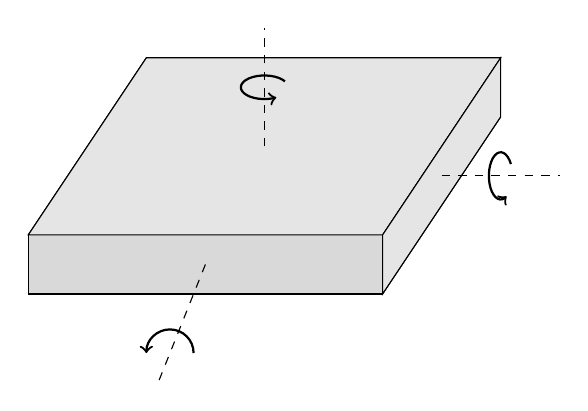
\begin{tikzpicture}[scale=1.5]
		% Face avant
		\draw[fill=gray!30] (0,0) rectangle (3,0.5);
		
		\draw (0,0.5) -- (1,2);
		\draw (3, 0.5) -- (4,2);
		\draw (3,0) -- (4,1.5);
		\draw (4,1.5) -- (4,2);
		\draw (1,2) -- (4,2);
		\draw[fill=gray!20] (0,0.5) -- (3,0.5) -- (4,2) -- (1,2) -- cycle;
		\draw[fill=gray!20] (3,0) -- (3,0.5) -- (4,2) -- (4,1.5) -- cycle;
		\draw[dashed] (2, 1.25) -- (2, 2.25);
		\draw[dashed] (3.5, 1) -- (4.5,1);
		\draw[dashed] (1.5,0.25) -- (1.1,-0.75);
		\draw[thick, ->] (1.4,-0.5) arc[start angle=0,end angle=180,radius=0.2];
		\draw [black, thick, domain=30:300, ->] plot ({2+0.2*cos(\x)}, {1.75+0.1*sin(\x)});
		\draw [black, thick, domain=30:300, ->] plot ({4+0.1*cos(\x)}, {1+0.2*sin(\x)});
	\end{tikzpicture}

	\begin{figure}[H]
		\caption{LSM9DS1 axis  on this card}
	\end{figure}
	
\end{center}

\section{Specification}

\subsection{Accelerometer Sensor}

The accelerometer is composed by sensor type MEMS (Micro-Electro-Mechanical Systems) and they used microscopic structures like suspended beams or springs, which deform in response to acceleration. The deformation of these structures is measured using displacement sensors or changes in electrical resistance. MEMS accelerometers are commonly used due to their small size, low power consumption, and comparatively lower cost compared to other types of accelerometers. \cite{pcb_mem_accelerometer:2024}

\bigskip 

The Accelerometer sensor function by \cite{mouser_memssensors:2024} : 

\begin{itemize}
	\item Acceleration Integration for Velocity Estimation: To estimate velocity, the acceleration measured by the accelerometer is integrated over time. Integrating acceleration over time yields velocity.
	
	\item Error Compensation: However, it's crucial to note that acceleration integration is susceptible to cumulative errors. Errors stemming from sensor noise, drift, and inaccuracies can accumulate over time, leading to inaccurate or biased velocity estimates.
	
	\item Utilization of Filters and Sensor Fusion Techniques: To compensate for these errors, advanced techniques such as Kalman filters, Complementary filters, or sensor fusion techniques can be employed. These techniques combine accelerometer data with other sensors such as gyroscopes to enhance velocity estimation accuracy.
	
	\item Calibration and Adjustment: It's also vital to calibrate and adjust the IMU to correct systematic errors and ensure precise measurements. This may involve steps such as compensating for Earth's gravity, correcting gyroscope drift, and reducing sensor noise. 
	
\end{itemize}
\subsection{PIN Conncetion}

They are 4 ways to connect pin, ways depend of what they have after \cite{st_microelectronics_lsm6dso32x:2024}. 

\begin{itemize}
	\item Mode 1: You can utilize either the I\textsuperscript{2}C / MIPI I3CSM slave interface or the SPI (3- and 4-wire) serial interface.
	
	\item Mode 2: This mode supports both the I\textsuperscript{2}C / MIPI I3CSM slave interface or the SPI (3- and 4-wire) serial interface, along with an I\textsuperscript{2}C interface master for external sensor connections.
	
	\item Mode 3: Here, you have the choice of employing either the I\textsuperscript{2}C / MIPI I3CSM slave interface or the SPI (3- and 4-wire) serial interface for the application processor interface. Additionally, an auxiliary SPI (3- and 4-wire) serial interface is designated for external sensor connections, exclusively for the gyroscope.
	
	\item Mode 4: Similar to Mode 3, this mode offers the I\textsuperscript{2}C / MIPI I3CSM slave interface or the SPI (3- and 4-wire) serial interface for the application processor interface. Additionally, it provides an auxiliary SPI (3- and 4-wire) serial interface for external sensor connections, catering to both the accelerometer and gyroscope.	
	
\end{itemize}

\begin{figure}[H]
	\begin{center}
		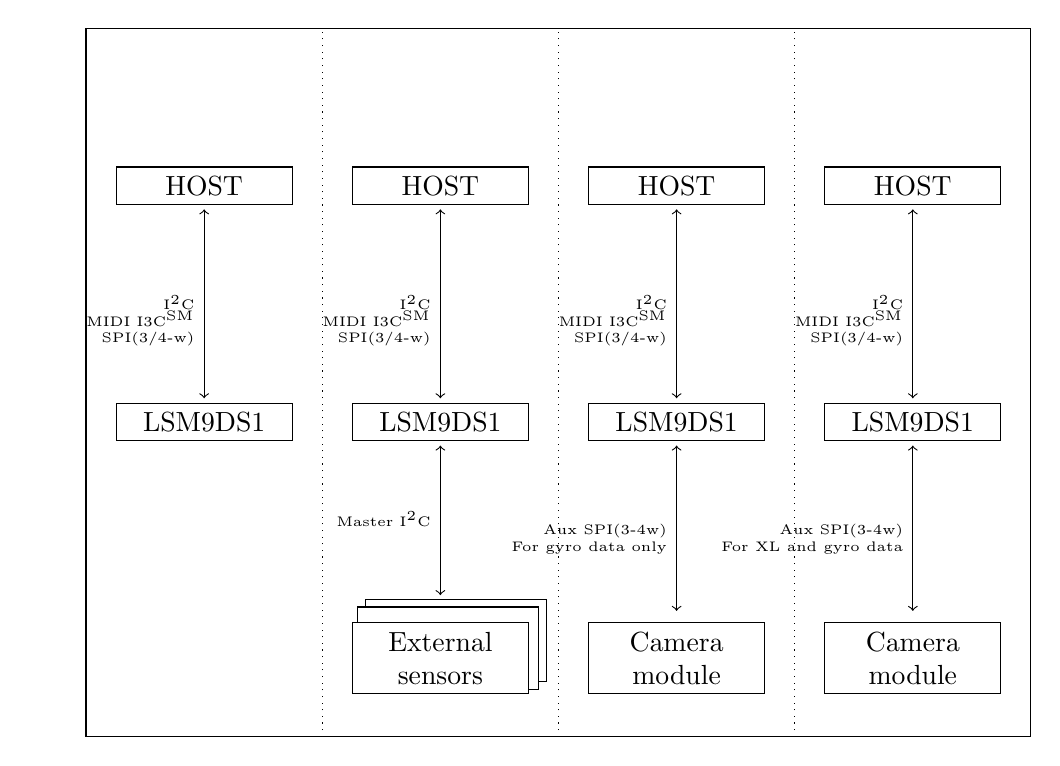
\begin{tikzpicture}
			\draw[fill=white] (0,0) rectangle++(12,9);
			\foreach \x in {3,6,9}{
			\draw[dotted] (\x, 0) -- (\x, 9);}
			\foreach \x in {1.5,4.5,7.5,10.5}{
			\node[draw, fill=white!20, text width=2cm, align=center] at (\x,7) {HOST};
			\node[draw, fill=white!20, text width=2cm, align=center] at (\x,4) {LSM9DS1};}
			\foreach \x in {1.5,4.5,7.5,10.5}{
			\draw[<->](\x,4.3) -- (\x,6.7) node[midway, anchor = mid east, align = right, text width = 2cm, font=\tiny]{I\textsuperscript{2}C\\ MIDI I3C\textsuperscript{SM}\\SPI(3/4-w)};}
			\foreach \x in {7.5,10.5}{
			\node[draw, fill=white!20, text width=2cm, align=center] at (\x,1) {Camera module};
			\draw[<->](\x,1.6) -- (\x,3.7) node[midway, anchor = mid east, align = right, text width = 2cm, font=\tiny]{Aux SPI(3-4w)};}
			\node[anchor=east, align= left, font=\tiny] at (7.5,2.4) {For gyro data only};
			\node[anchor=east,  align= left, font=\tiny] at (10.5,2.4) {For XL and gyro data};
			\draw[fill=white] (3.55,0.7) rectangle++(2.3, 1.05) ;
			\draw[fill=white] (3.45,0.6) rectangle++(2.3, 1.05) ;
			\node[draw, fill=white!20, text width=2cm, align=center] at (4.5,1) {External sensors};
			\draw[<->](4.5,1.8) -- (4.5,3.7) node[midway, anchor = mid east, align = right, text width = 2cm, font=\tiny]{Master I\textsuperscript{2}C};
				
		\end{tikzpicture}
		\caption{Explication of pin mode}  
	\end{center}
\end{figure}

\section{Libraries}

\subsection{Library Description}

\begin{enumerate}
	\item \FILE{Wire.h} : 	This library is a standard Arduino library that facilitates communication between I\textsuperscript{2}C (Inter-Integrated Circuit) devices. I\textsuperscript{2}C is a synchronous serial communication protocol used to connect microcontrollers to external devices. \FILE{Wire.h} provides functions for initializing the I\textsuperscript{2}C bus, sending and receiving data on the bus, and managing multiple devices on the same bus. With this library, developers can easily connect multiple I\textsuperscript{2}C devices, such as sensors or displays, to an Arduino board. \cite{arduino_wire:2024}
	
	\item \FILE{Kalman.h} : It's a library that implements the Kalman filter algorithm. The Kalman filter is a mathematical technique used to estimate the state of a system from incomplete measurements. It is commonly used in control systems, robotics and navigation applications to improve the accuracy of sensor measurements and reduce errors. \FILE{Kalman.h} provides a simple interface for developers to implement the Kalman filter in their Arduino projects. \cite{arduino_kalman:2024}

	\item \FILE{Arduino LSM9DS1.h} :
	The LSM9DS1 library is a software library designed to facilitate interaction with the LSM9DS1 inertial sensor, developed by STMicroelectronics. This sensor combines an accelerometer, a gyroscope and a magnetometer in a single package.The LSM9DS1 library provides an interface for accessing the sensor's functionalities, such as reading acceleration, angular velocity and magnetic field data. It can be used to configure various sensor parameters, such as measurement scales, sampling rates and operating modes. \cite{arduino_lsm9ds1:2024}
	
	
\end{enumerate}

\subsection{Installation}

The bibliographie give coding example for used it, we need to download Arduino Library.  The library \FILE{Arduino LSM9DS1.h} and \FILE{Kalman.h} can be download directly on Arduino. The library \FILE{wire.h} is used if you imput :  include <wire.h>

	\begin{center}
		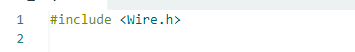
\includegraphics[width=0.7\linewidth]{Images/ArduinoIDE/wire.png}
		\captionof{figure}{Wire include} 
	\end{center}



	\begin{center}
		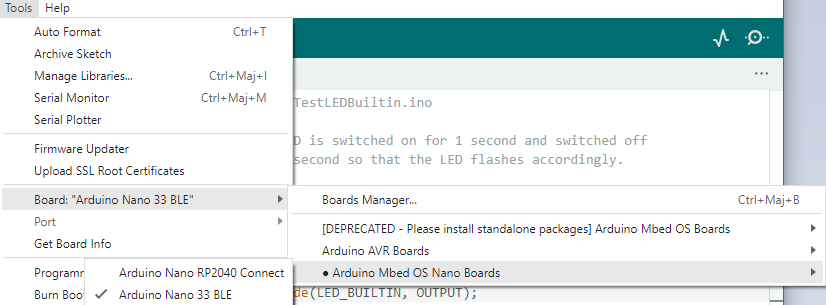
\includegraphics[width=0.7\linewidth]{Images/ArduinoIDE/LSM6DSboard.png}
		\captionof{figure}{Board card installation}
	%	\bigskip
	\end{center}


	\begin{center}	
		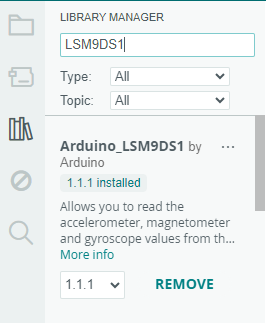
\includegraphics[width=0.7\linewidth]{Images/ArduinoIDE/LSM9DS1.png}
		\captionof{figure}{Library choice}
	\end{center}


	\bigskip



\section{Function}

The LSM9DS1 library on Arduino PortentaH7 is composed of different function. The function is different if you was on I\textsuperscript{2}C protocol or SPI protocol.
 

\bigskip


\lstdefinestyle{Arduino}{
	language=Arduino,
	basicstyle=\ttfamily\small,
	keywordstyle=\color{blue},
	stringstyle=\color{yellow!30!black},
	commentstyle=\color{green!60!blue},
	morecomment=[l]{//},
	morecomment=[s]{/*}{*/} }

\subsection{Library \FILE{Wire.h}}


This library is used to devellop communication betwin different composent of arduino, it's used for I\textsuperscript{2}C. Wire.h is composed by  \cite{arduino_wire:2024} : 
\begin{itemize}
	
	\item \PYTHON{Wire.begin()}: Initializes the Wire library and prepares the Arduino to act as master or slave on the bus I\textsuperscript{2}C.
	\item \PYTHON{Wire.beginTransmission(address)}: Starts a transmission to a slave device with the specified address.
	\item \PYTHON{Wire.write(data)} : Sends data on the I2C bus during transmission.
	\item \PYTHON{Wire.endTransmission()} : Ends the current transmission and releases the I2C bus.
	\item \PYTHON{Wire.requestFrom(address, quantity)} : Requests data from a slave device with the specified address.
	\item \PYTHON{Wire.available()}: Checks whether data is available to be read after a request.
	\item \PYTHON{Wire.read()}: Reads data received from a slave device.

\end{itemize}


\begin{code}
	\lstinputlisting[language=python]{../Code/Arduino/IMU/WireEx.ino}
	
	 \caption{Simple sketch using the sensor LSM9DS1 detection.}\label{TestWire}
	 
\end{code}


\subsection{Function \PYTHON{IMU.begin()}}


Calling the function triggers  \PYTHON{IMU.begin()}, the IMU initialization process. This step is important to configures the IMU's basic parameters, establishes communications with other devices, and prepares the unit for proper operation. Accurate initialization is essential to ensure the accuracy and reliability of the data provided by the IMU. \cite{arduino_lsm9ds1:2024}

Incorrect initialization can lead to inaccurate measurements or unpredictable behavior. For example, incorrectly configured measurement parameters or sampling rates can compromise data quality, affecting overall system performance.


\begin{lstlisting}[style= Arduino]
	if (!IMU.begin()) {
		Serial.println("Failed to initialize IMU!");
		while (1);	}
\end{lstlisting}


\subsection{Function \PYTHON{IMU.end()}} 

No parameters is required. A return value of 1 indicates that all went well, while a return value of 0 indicates a problem. \cite{arduino_lsm9ds1:2024}

This function is used to stop or deactivate the IMU once it is no longer required. It frees up the resources used by the IMU and ends its operation cleanly. When called, it ensures that all tasks associated with the IMU are properly finalized, avoiding memory leaks or other problems associated with incomplete de-initialization.

This step helps to ensure the stability and reliability of the system as a whole, by avoiding problems associated with incorrect IMU de-initialization.

The data was return at the end. 

\begin{lstlisting}[style=Arduino]
	if (!IMU.begin()) {
		Serial.println("Failed to initialize IMU!");
		while (1); }
			
\end{lstlisting}


\subsection{Function \PYTHON{IMU.readAcceleration(x,y,z) }}

IMU accelerometer to retrieve acceleration data, expressed in gravity (g). This function provides information on the movements detected by the IMU's accelerometer. The resulting acceleration data can be used for a variety of applications, such as shock or motion detection, or inertial navigation. By regularly interrogating the accelerometer and analyzing variations in acceleration, it is possible to understand and react to changes in motion with precision, which is essential in many modern embedded systems and electronic devices. \cite{adafruit_lsm9ds1:2024}

The parameters x, y and z are floats giving information on the x, y or z axis 

\begin{lstlisting}[style=Arduino]
	
	float x, y, z;
	
	if (IMU.accelerationAvailable()) {
		IMU.readAcceleration(x, y, z);
		
		Serial.print(x);
		Serial.print('\t');
		Serial.print(y);
		Serial.print('\t');
		Serial.println(z);	}
\end{lstlisting}



\subsection{Function \PYTHON{IMU.readGyroscope()}}

Retrieves data from the IMU's gyroscope and returns angular velocity in degrees per second (dps). This function provides information on the rotational movement detected by the IMU's gyroscope. The angular velocity data retrieved can be used in various applications such as robotics, motion tracking or navigation systems. By regularly interrogating the gyroscope and analyzing angular velocity variations, it becomes possible to understand and respond precisely to rotational movements, which is crucial in applications requiring precise orientation control or stabilization. \cite{adafruit_lsm9ds1:2024}

The parameters x, y and z are floats giving information on the x, y or z axis 

\begin{lstlisting}[style=Arduino]
	float x, y, z;
	
	if (IMU.gyroscopeAvailable()) {
		IMU.readGyroscope(x, y, z);
		
		Serial.print(x);
		Serial.print('\t');
		Serial.print(y);
		Serial.print('\t');
		Serial.println(z);	}
\end{lstlisting}



\subsection{Function \PYTHON{IMU.accelerationAvailable()}}

This function allows you to check the status of IMU acceleration data, indicating whether or not new data is ready to be retrieved.

In scenarios such as motion tracking, robotics or navigation systems, where the IMU continuously captures acceleration data, the availability of new data determines the system answers. Test the IMU at regular intervals is used for application and they can check for acceleration currently or non, ensuring that the system remains synchronized with object movements in real time. \cite{adafruit_lsm9ds1:2024}

When the function returns a value of 1, this means that new acceleration data is available, enabling the system to extract the data and process it further. A value of 0 indicates that there have been no recent acceleration updates.

\begin{lstlisting}[style=Arduino]
	float x, y, z;
	
	if (IMU.accelerationAvailable()) {
		IMU.readAcceleration(x, y, z);
		
		Serial.print(x);
		Serial.print('\t');
		Serial.print(y);
		Serial.print('\t');
		Serial.println(z); }

\end{lstlisting}


\subsection{Function \PYTHON{IMU.gyroscopeAvailable()}}

This function ask if new gyro data are available for the IMU and they returns a value 0 if no new gyro data is available, and 1 if new gyro data is ready to be retrieved.

In applications requiring real-time monitoring of rotational motion, such as drone stabilization, virtual reality systems or inertial navigation, the system can determine whether to wait for updated gyroscope readings or proceed to process available data. \cite{Arduino_IMU_Gyroscope:2024}

A value of 1 indicates that new gyro data is available, enabling the system to retrieve and use this information for adapted the orientation tracking or motion control. Conversely, a feedback value of 0 indicates that there have been no recent updates to the gyroscope measurements, prompting the system to wait for new data to become available before proceeding.

\begin{lstlisting}[style=Arduino]
	float x, y, z;
	
	if (IMU.gyroscopeAvailable()) {
		IMU.readGyroscope(x, y, z);
		
		Serial.print(x);
		Serial.print('t');
		Serial.print(y);
		Serial.print(' t');
		Serial.println(z); }
\end{lstlisting}


\subsection{Function \PYTHON{IMU.accelerationSampleRate()}}

This function is designed to provide information on the sampling rate of the IMU's accelerometer. The function \PYTHON{IMU.accelerationSampleRate()} returns the accelerometer sampling rate, expressed in Hertz (Hz). This value represents the frequency at which the accelerometer takes measurements and provides acceleration data. It indicates how many times per second the accelerometer registers changes in acceleration along its axes. \cite{STMicroelectronics_LSM9DS1:2024}

In activities such as motion tracking, gesture recognition or vibration analysis, knowledge of the accelerometer's sampling rate ensures that the system can accurately capture and respond to changes in motion dynamics. 

\begin{lstlisting}[style=Arduino]
	Serial.print("Accelerometer sample rate = ");
	Serial.print(IMU.accelerationSampleRate());
	Serial.println(" Hz");
	Serial.println();
	Serial.println("Acceleration in g's");
	Serial.println("X \t Y  \t Z");
\end{lstlisting}



\subsection{Function \PYTHON{IMU.gyroscopeSampleRate()}}

To recover and communicate the specific rate at which the gyroscope, integrated into the inertial measurement unit (IMU), collects data samples. This frequency is usually expressed in hertz (Hz), corresponding to the number of samples acquired per second. This is the frequency at which the gyroscope takes measurements, giving an idea of its operational efficiency and performance. \cite{STMicroelectronics_LSM9DS1:2024}

\begin{lstlisting}[style=Arduino]
	Serial.print("Gyroscope sample rate = ");
	Serial.print(IMU.gyroscopeSampleRate());
	Serial.println(" Hz");
	Serial.println();
	Serial.println("Angular speed in degrees/second");
	Serial.println("X tY tZ");
	
\end{lstlisting}

